\documentclass[tikz,border=2mm]{standalone}
\usepackage{pgfplots}
\pgfplotsset{compat=1.18}
\begin{document}
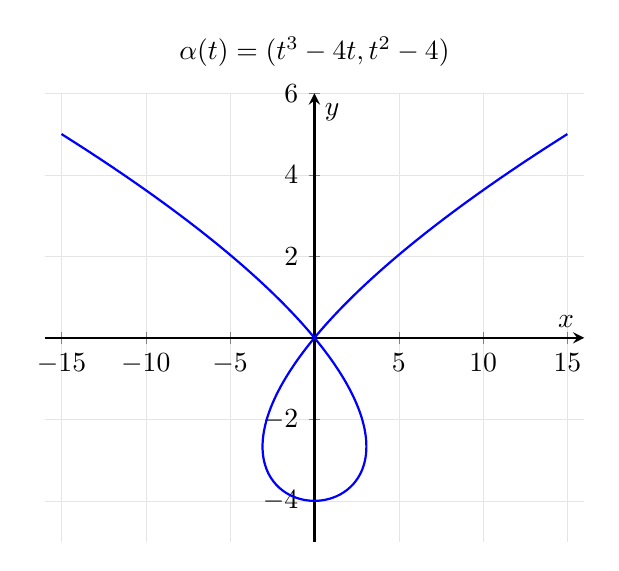
\begin{tikzpicture}
\begin{axis}[
    title={$\alpha(t)=(t^3-4t, t^2-4)$},
    axis lines=middle,
    xlabel={$x$},
    ylabel={$y$},
    xmin=-16, xmax=16,
    ymin=-5, ymax=6,
    domain=-3:3,
    samples=100,
    grid=both,
    grid style={line width=.1pt, draw=gray!20},
    thick
]
\addplot[blue, smooth, variable=\t] ({t^3 - 4*t}, {t^2 - 4});
\end{axis}
\end{tikzpicture}
\end{document}
